\documentclass[a4paper,11pt]{article}
\title{PAG Ionisation energy of a thermistor}
\author{Izaak van Dongen}

% so the title can be accessed by fancyhdr (and is automatically correctly
% spelled etc)
\makeatletter
\let\thetitle\@title
\makeatother

% fonts
\usepackage[p,osf]{cochineal}
\usepackage[scale=.95,type1]{cabin}
\usepackage[cochineal,bigdelims,cmintegrals,vvarbb]{newtxmath}
% fixed width font with 80 chars per listing line
\usepackage[scaled=.94]{newtxtt}
\usepackage[cal=boondoxo]{mathalfa}

% make the document take up more of the page
\usepackage[margin=1in,headheight=13.6pt]{geometry}

% no paragraph indent
\usepackage[parfill]{parskip}

% custom document header/footer
\usepackage{fancyhdr}
\usepackage{lastpage}

\pagestyle{fancy}
\fancyhf{}
\lhead{\thetitle}
\rhead{Izaak van Dongen}
\rfoot{Page \thepage\ of \pageref{LastPage}}

% pretty table rules and multirow entries. Also page-breaking tables
\usepackage{booktabs}
\usepackage{multirow}
\usepackage{longtable}

% plotting mathematical functions (needs version request)
\usepackage{pgfplots}
\pgfplotsset{compat=1.15}

% \url function and clickable table of contents. no ugly red boxes though
\usepackage[hidelinks]{hyperref}

% maths symbols and other stuff (supersedes the ams* packages)
\usepackage{mathtools}

% For framing definitions
\usepackage[framemethod=tikz]{mdframed}
\usepackage[most]{tcolorbox}

\newtcolorbox{definition}{
freelance,
before=\par\vspace{2\bigskipamount}\noindent,
after=\par\bigskip,
frame code={
  \node[
  anchor=south west,
  inner xsep=8pt,
  xshift=8pt,
  rounded corners=5pt,
  font=\bfseries\color{white},
  fill=gray] at (frame.north west) (tit) {\strut Definition:};
  \draw[
  line width=3pt,
  rounded corners=5pt,gray
  ] (tit.west) -| (frame.south west) -- ([xshift=15pt]frame.south west);
},
interior code={},
top=2pt
}

% for better table of contents stuff, providing the \listof* commands and not
% listing the tables in the table of contents
\usepackage[nottoc,notlof,notlot]{tocbibind}

% more advanced handling of utf8 and fonts or something. apparently good to have
\usepackage[utf8]{inputenc}
\usepackage[T1]{fontenc}

% bibliography management with square braces for citations
\usepackage[square,numbers]{natbib}

% graphics, like eps files and stuff (supersedes graphics)
\usepackage{graphicx}

% used to horizontally align floats
\usepackage{subfig}

% used for figures
\usepackage{float}

% needed for colouring and stuff (xcolor supersedes color)
\usepackage{xcolor}

\definecolor{codegreen}{rgb}{ 0,0.6,0}

% listings of code
\usepackage{minted}
\setminted{breaklines,
           breakbytokenanywhere,
           linenos
}
\usemintedstyle{friendly}
% bigger line numbers
\renewcommand\theFancyVerbLine{\footnotesize\arabic{FancyVerbLine}}

% that can break across pages while being captioned figures
\usepackage{caption}
\newenvironment{longlisting}
{\addvspace{\baselineskip}\captionsetup{type=listing}}
{\addvspace{\baselineskip}}

% allow maths to break across pages
\allowdisplaybreaks

\usepackage{siunitx}

\begin{document}
    \maketitle%\thispagestyle{empty} % no page number under title

\begin{longlisting}
\inputminted{R}{analyse.r}
\caption{R source}
\end{longlisting}

\begin{longlisting}
\begin{minted}{text}
[1] 5.1525
[1] 0.01818182
[1] 0.0006685609
   T_celsius I_ma      T       I     T_recip      ln_I
1          9 0.28 282.15 0.00028 0.003544214 -8.180721
2         10 0.29 283.15 0.00029 0.003531697 -8.145630
3         11 0.30 284.15 0.00030 0.003519268 -8.111728
4         12 0.31 285.15 0.00031 0.003506926 -8.078938
5         13 0.33 286.15 0.00033 0.003494671 -8.016418
6         14 0.34 287.15 0.00034 0.003482500 -7.986565
7         15 0.35 288.15 0.00035 0.003470415 -7.957577
8         16 0.37 289.15 0.00037 0.003458413 -7.902008
9         17 0.39 290.15 0.00039 0.003446493 -7.849364
10        18 0.40 291.15 0.00040 0.003434656 -7.824046
11        19 0.42 292.15 0.00042 0.003422899 -7.775256
12        20 0.43 293.15 0.00043 0.003411223 -7.751725
13        21 0.45 294.15 0.00045 0.003399626 -7.706263
14        22 0.47 295.15 0.00047 0.003388108 -7.662778
15        23 0.48 296.15 0.00048 0.003376667 -7.641724
16        24 0.51 297.15 0.00051 0.003365304 -7.581100
17        25 0.53 298.15 0.00053 0.003354016 -7.542634
18        26 0.55 299.15 0.00055 0.003342805 -7.505592
19        27 0.57 300.15 0.00057 0.003331667 -7.469874
20        28 0.59 301.15 0.00059 0.003320604 -7.435388
21        29 0.61 302.15 0.00061 0.003309614 -7.402052
22        30 0.63 303.15 0.00063 0.003298697 -7.369791
23        31 0.66 304.15 0.00066 0.003287851 -7.323271
24        32 0.68 305.15 0.00068 0.003277077 -7.293418
25        33 0.70 306.15 0.00070 0.003266373 -7.264430
26        34 0.73 307.15 0.00073 0.003255738 -7.222466
27        35 0.75 308.15 0.00075 0.003245173 -7.195437
28        36 0.78 309.15 0.00078 0.003234676 -7.156217
29        37 0.81 310.15 0.00081 0.003224246 -7.118476
30        38 0.84 311.15 0.00084 0.003213884 -7.082109
31        39 0.87 312.15 0.00087 0.003203588 -7.047017
32        40 0.89 313.15 0.00089 0.003193358 -7.024289
33        41 0.93 314.15 0.00093 0.003183193 -6.980326
34        42 0.96 315.15 0.00096 0.003173092 -6.948577
35        43 1.01 316.15 0.00101 0.003163056 -6.897805
Nonlinear regression model
  model: I ~ A * exp(-E/(k * T))
   data: current_df
        A         E
4.003e+01 4.627e-20
 residual sum-of-squares: 6.51e-10

Number of iterations to convergence: 11
Achieved convergence tolerance: 2.081e-06

Call:
lm(formula = ln_I ~ T_recip, data = current_df)

Coefficients:
(Intercept)      T_recip
      3.695    -3353.201
\end{minted}
\caption{Model results}
\end{longlisting}

\begin{figure}[H]
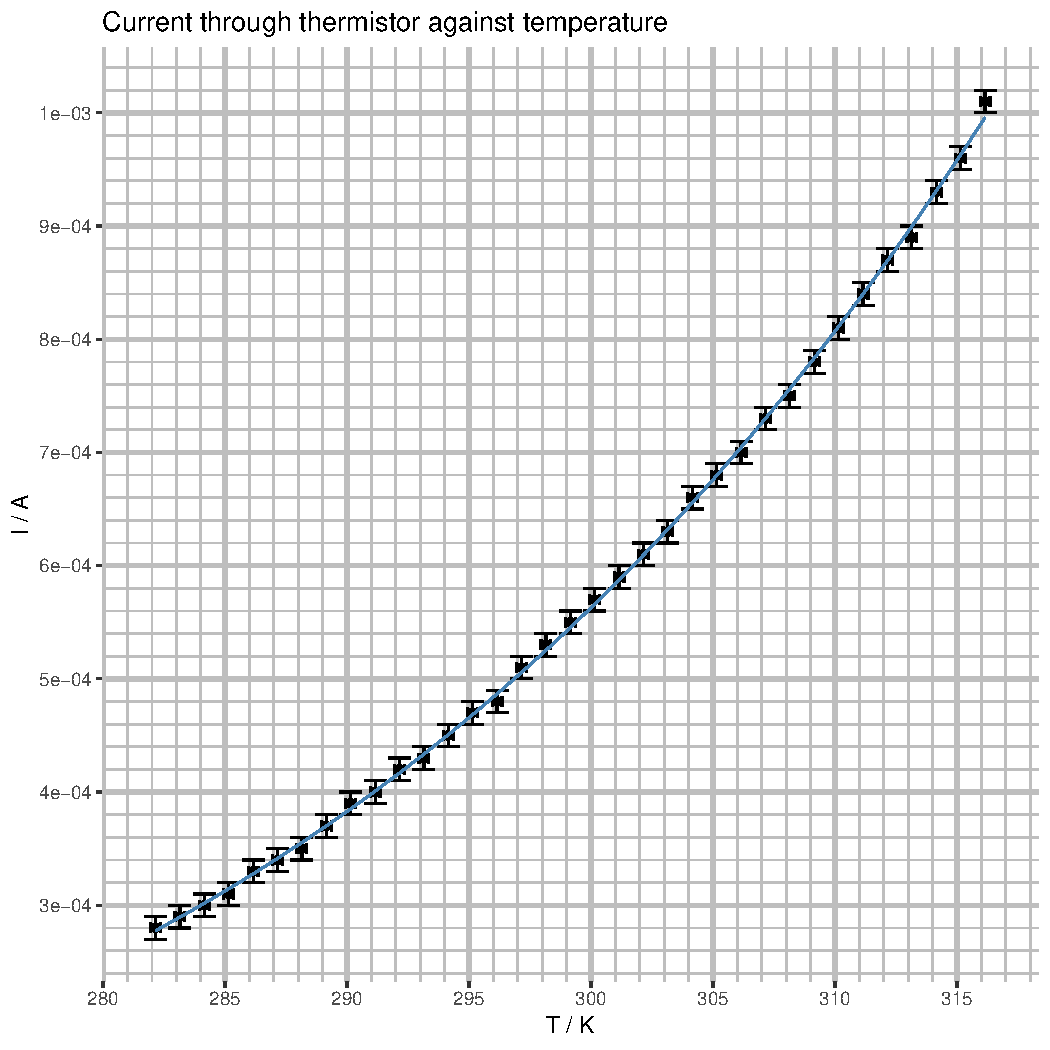
\includegraphics[width=\textwidth,page=1]{Rplots.pdf}
\caption{Graph of $I/A$ against $T/K$}
\label{fig:nonlinear}
\end{figure}

\begin{figure}[H]
\includegraphics[width=\textwidth,page=2]{Rplots.pdf}
\caption{Linearised graph $\ln{I} - \ln{A}$ against $K/T$}
\label{fig:linear}
\end{figure}

The nonlinear regression in figure \ref{fig:nonlinear} found a value for
$\varepsilon$ as \SI{4.627e-20}{\joule}.

The linear regression in figure \ref{fig:linear} found
$-\frac{\varepsilon}{k} = \SI{-3353.201}{\kelvin}
\Rightarrow \varepsilon = 3353.201 \times \SI{1.381e-23}{\joule}
= \SI{4.629e-20}{\joule}
$

So $\varepsilon = \SI{4.63e-20}{\joule}$ to 3 SF is consistent with both
analyses.

Alternatively expressed,
$\varepsilon = \SI{0.290}{e\volt} = \SI{27.9}{\kilo\joule\per\mol}
             \approx 11kT$, where
$T = \SI{300}{\kelvin}$.

\end{document}
